\documentclass[10pt, conference, a4paper, final]{IEEEtran}
\IEEEoverridecommandlockouts
% For better handling of math expressions
\usepackage{amsmath}

% For better formatting of lists
\usepackage{enumitem}

% Optional for improved typography
\usepackage{microtype}
\usepackage[margin=1in]{geometry} % Adjust margins as needed
\usepackage{lipsum} % Provides sample text. Remove this for your actual document.
\usepackage[table,xcdraw]{xcolor}
\usepackage{colortbl}
\usepackage{graphicx} % Required for including images
\usepackage{graphicx}
\usepackage{textcomp}
\usepackage{xcolor}
\usepackage{float}
\usepackage{amsmath}
\usepackage{longtable}
\usepackage{booktabs}
\usepackage{multicol}
\usepackage{multirow}
\usepackage{relsize, fullpage, url, array}
\usepackage{lscape, afterpage}
\usepackage{float,lscape}
\usepackage{algorithm}
\usepackage{algorithmic}  
\usepackage[algo2e]{algorithm2e} 
\usepackage{amsmath}
\usepackage{mathtools}
\usepackage{tabularx}
\usepackage{algorithmic}
\usepackage{graphicx}
\usepackage{textcomp}
\usepackage{xcolor}
\title{Beyond Accuracy: Evaluating Deep Learning Robustness in Adversarial Environments}
\author{Arooj Arif}
\date{\today} % You can also specify a date manually

\begin{document}

\maketitle % This command creates the title

\section{Introduction and Background:}


The document opens with an introduction to adversarial machine learning (AML), emphasizing its growing importance in the field of artificial intelligence. It explains that AML studies the vulnerabilities of machine learning systems to adversarial attacks and the corresponding defenses.
The necessity of a taxonomy for AML is outlined, highlighting the need for a structured way to classify and understand different types of attacks and defenses. This taxonomy aids in establishing a common language and understanding in the rapidly evolving field of AML.
\section{Classification and Description of Adversarial Attacks:}

The taxonomy categorizes attacks based on various dimensions such as the learning method, the stage of the learning process during which the attack occurs, the goals and objectives of the attacker, their capabilities, and their knowledge of the learning process.
Attack Objectives: The document classifies attacker objectives into three main categories: availability breakdown, integrity violations, and privacy compromise. These objectives form the core of the taxonomy and are used to structure the classification of different attacks.
Attacker Capabilities: The capabilities of an attacker are diverse, ranging from control over training or testing data to control over the model parameters or source code of the ML algorithms.
\section{Learning Paradigms and Stages:}

The document discusses various machine learning paradigms, including supervised, unsupervised, semi-supervised, reinforcement, federated, and ensemble learning, and how they are impacted by adversarial attacks.
It also distinguishes between attacks occurring at different stages of machine learning: during the training stage (poisoning attacks) and the deployment stage (evasion and privacy attacks).
\section{Attack Methodologies:}
\begin{figure*}[!ht]
    \centering
    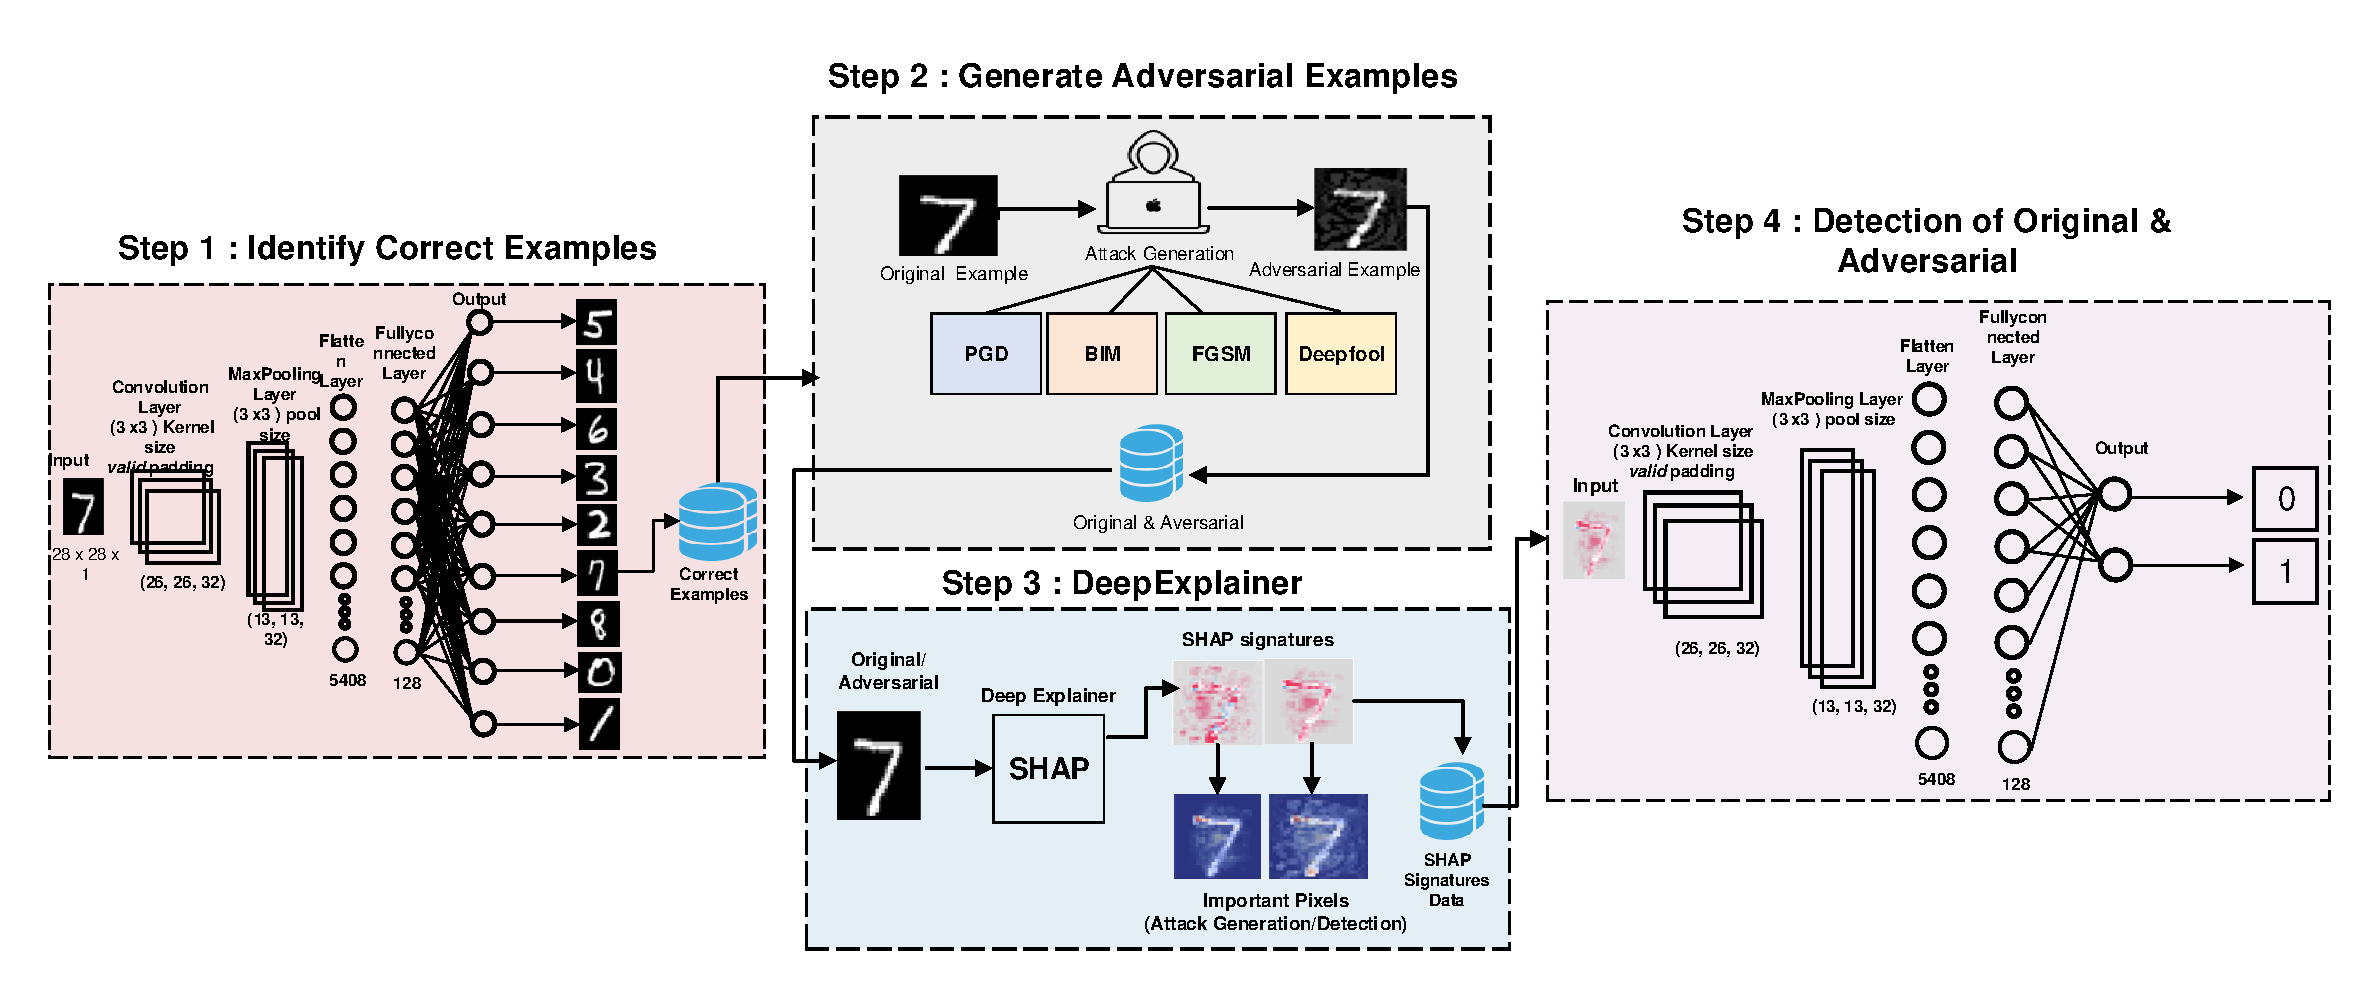
\includegraphics[width=1\textwidth]{paper_images/conference_model.pdf}
    \caption{Threat Model}
    \label{threat model}
    \end{figure*}
Detailed methodologies of different types of attacks are presented, including data poisoning attacks during training and evasion attacks during deployment. Specific examples and techniques used in these attacks are discussed to provide a clear understanding of how they are executed.
\section{Mitigation Strategies:}

The document outlines various strategies and methods for mitigating the impacts of adversarial attacks. These strategies are essential for enhancing the security and robustness of machine learning systems against adversarial threats.
\section{Case Studies and Applications:}

\subsection{Case Study 1: Epsilon Sensitivity Analysis}
Objective: To analyze how different levels of epsilon affect model performance.
Method: Compare the rate of successful adversarial examples (i.e., success) across different epsilons for each attack.
Analysis: You can plot the success rate against epsilon to visualize the relationship. A steep increase at lower epsilon values might suggest that the model is highly sensitive to small perturbations.
\subsection{Case Study 2: Attack Specificity and Misclassification Patterns}
Objective: To examine if certain attacks are more successful on specific classes.
Method: Use the confusion matrices from each attack to see which true classes are most frequently misclassified and what they are misclassified as.
Analysis: You can identify whether some classes are consistently more vulnerable across attacks or if certain attacks are class-specific. Look for patterns in misclassifications — are there certain features or similarities in the data that make specific classes more prone to adversarial attacks?
\subsection{Case Study 3: Robust Accuracy Across Attacks}
Objective: To evaluate which type of attack the model is most robust against.
Method: Compare the robust accuracy for each attack type at various epsilon levels.
Analysis: This can reveal insights into the model’s relative robustness to different adversarial strategies. It’s particularly interesting to note if the model maintains high accuracy against one attack type but not others, which could suggest specific defense mechanisms are more effective.
\subsection{Case Study 4: Comparative Analysis of Attack Strategies}
Objective: To compare the effectiveness of iterative (PGD) versus single-step (FastGradientAttack) attacks and additive noise.
Method: Utilize the adversarial examples generated to assess the distortion introduced and the perceptibility of these perturbations.
Analysis: Compare the magnitude of changes required by each attack to successfully fool the model. Iterative attacks might introduce smaller, less perceptible changes, which could be more dangerous in real-world scenarios.
\begin{figure*}[!ht]
    \centering
    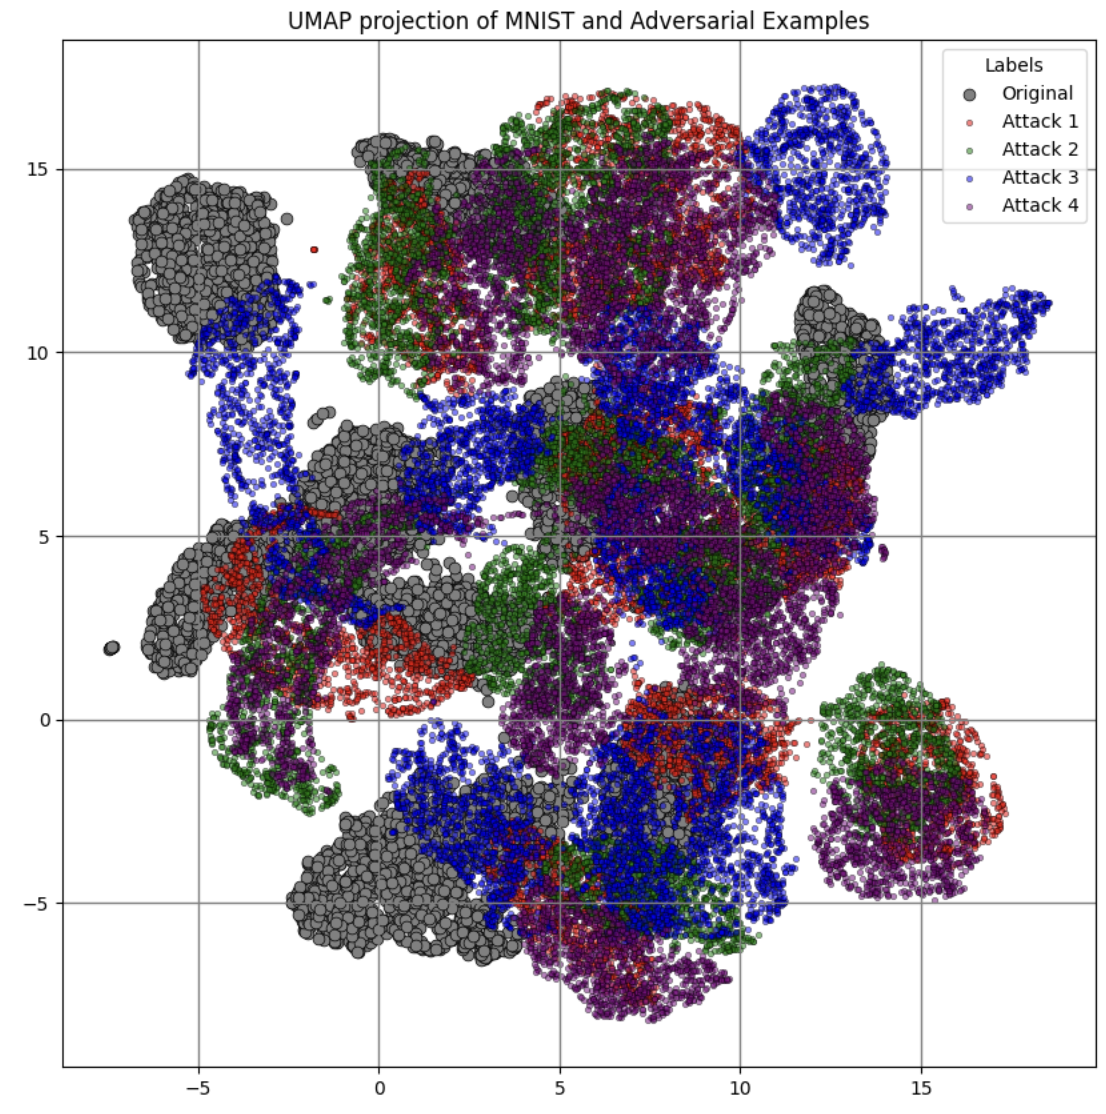
\includegraphics[width=0.5\textwidth]{paper_images/UMAP_adversary.png}
    \caption{Threat Model}
    \label{threat model}
    \end{figure*}
    \begin{figure*}[!ht]
        \centering
        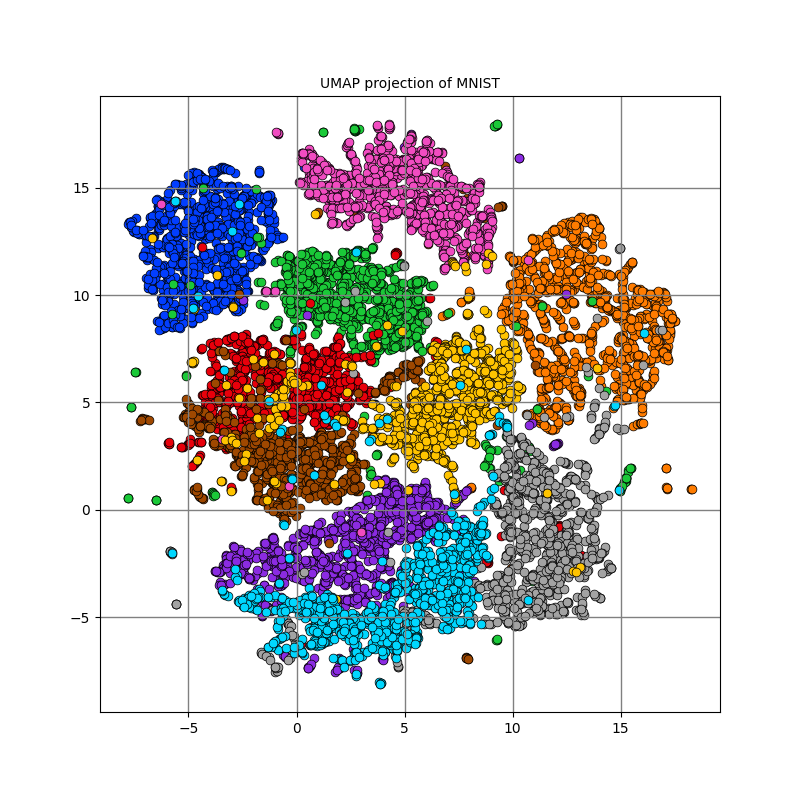
\includegraphics[width=0.5\textwidth]{paper_images/UMAPMNIST.png}
        \caption{Threat Model}
        \label{threat model}
        \end{figure*}

        \begin{figure*}[!ht]
            \centering
            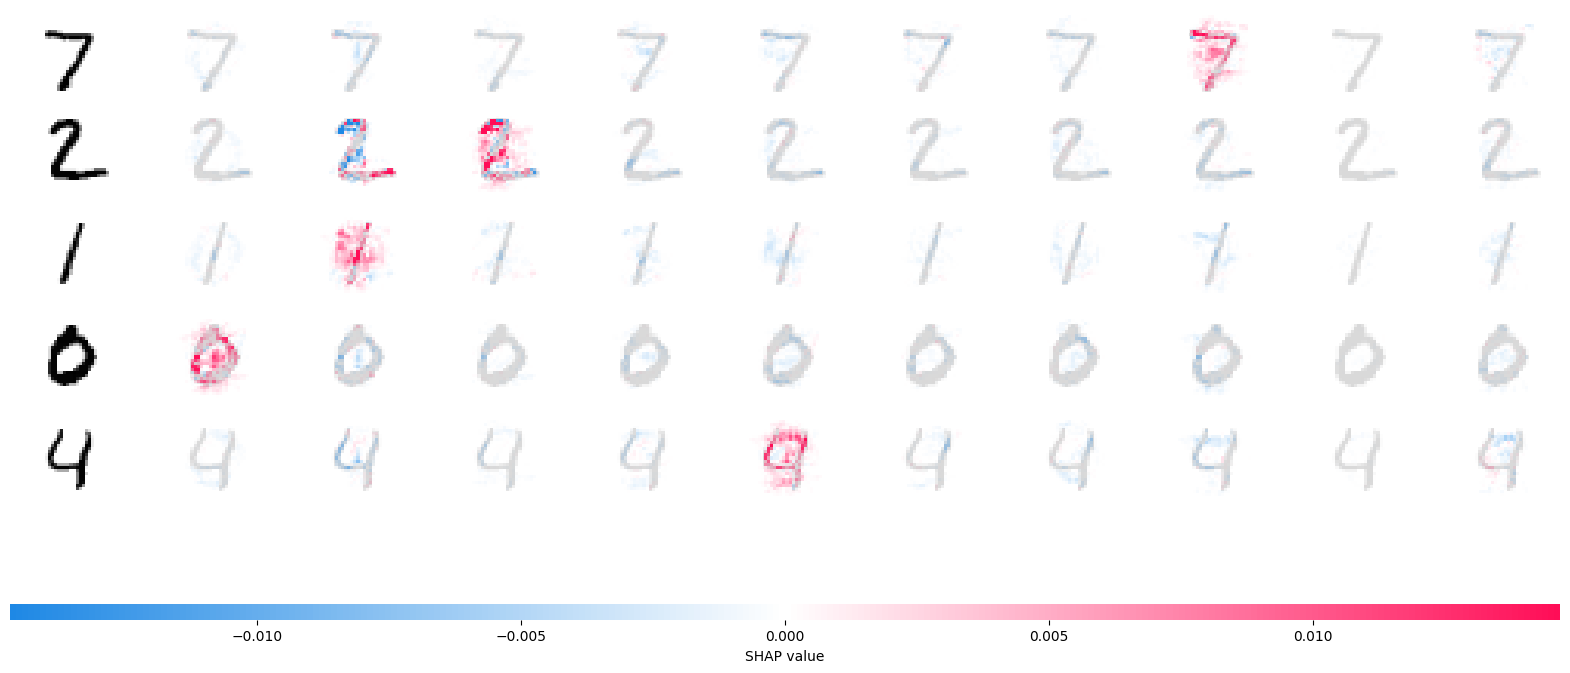
\includegraphics[width=1\textwidth]{paper_images/correctshap.png}
            \caption{Threat Model}
            \label{threat model}
            \end{figure*}
            \begin{figure*}[!ht]
                \centering
                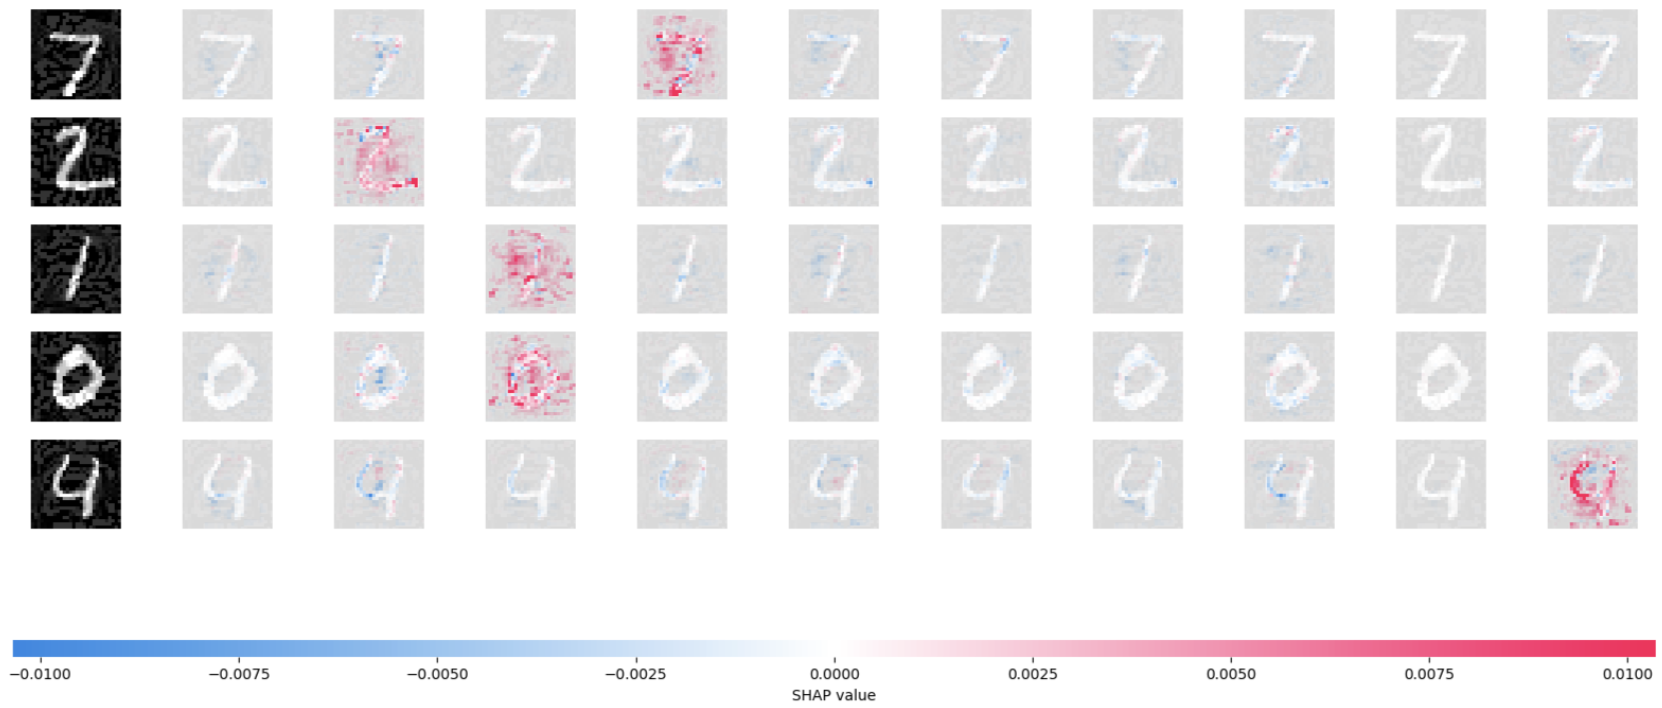
\includegraphics[width=1\textwidth]{paper_images/adversarial.png}
                \caption{Threat Model}
                \label{threat model}
                \end{figure*}
\section{Future Directions and Challenges:}

Further Research Directions:
Feature Importance Analysis:

Investigate what features of the input are most affected by adversarial perturbations. This could be done by analyzing gradients or using explainability tools like SHAP or LIME.
Transferability of Attacks:

Test if adversarial examples generated for one model are effective against another model. This would help understand the generalizability of adversarial examples.
Adversarial Training:

Incorporate adversarial examples into the training process to improve model robustness and then repeat the attacks to see if there’s an improvement.
Model Architecture Analysis:

Evaluate if changing the architecture (e.g., adding dropout, using different activation functions) affects robustness to adversarial attacks.
Human Perceptibility Study:

Conduct a user study to see if the perturbations generated at various epsilons are perceptible to the human eye. This is especially relevant for applications like facial recognition.
Defense Mechanism Testing:

Implement and test various defense mechanisms, such as input transformations (e.g., JPEG compression) or adversarial detection methods, and analyze their effectiveness against each type of attack.
\section{Conclusion:}

A summarization of the main findings and implications of the taxonomy is provided, emphasizing its importance in standardizing the understanding of adversarial attacks in machine learning.
This summary provides an overview of the key points and themes covered in the document. Due to the complexity and length of the document, each section contains a wealth of detailed information that is summarized here at a high level.
\begin{thebibliography}{01}

\bibitem{BR18}	
Battista Biggio and Fabio Roli. Wild patterns: Ten years after the rise of adversarial machine learning. Pattern Recognition, 84:317–331, 2018.


\end{thebibliography}
\end{document}
